\section{Auswertung}
\label{sec:Auswertung}
\subsection{Kennlinien der Diode}
Die aufgenommenen Werte lassen sich Tab. \ref{tab:Reihe1}, \ref{tab:Reihe2}, \ref{tab:Reihe3}, \ref{tab:Reihe4}, \ref{tab:Reihe4}, sowie Abb. \ref{fig:Plot1}, \ref{fig:Plot2}, \ref{fig:Plot3}, \ref{fig:Plot4} \ref{fig:Plot5}, entnehmen. Die Sättigungsströme ergeben sich so zu den in Tab. \ref{tab:Sett} dargestellten Werten.
\begin{table}
  \centering
  \caption{Sättigungsströme und zugehörige Heizleistungen}
  \label{tab:Sett}
  \begin{tabular}{|c|c|}
    \toprule
    $I/\si{\ampere}$ & $P_\symup{heiz}/\si{\watt}$ \\
    \midrule
    0.012 & 6.30 \\
    0.024 & 7.60 \\
    0.081 & 9.00 \\
    0.146 & 9.45 \\
    0.342 & 11.00 \\
    \bottomrule
\end{tabular}
\end{table}
\begin{figure}
  \centering
  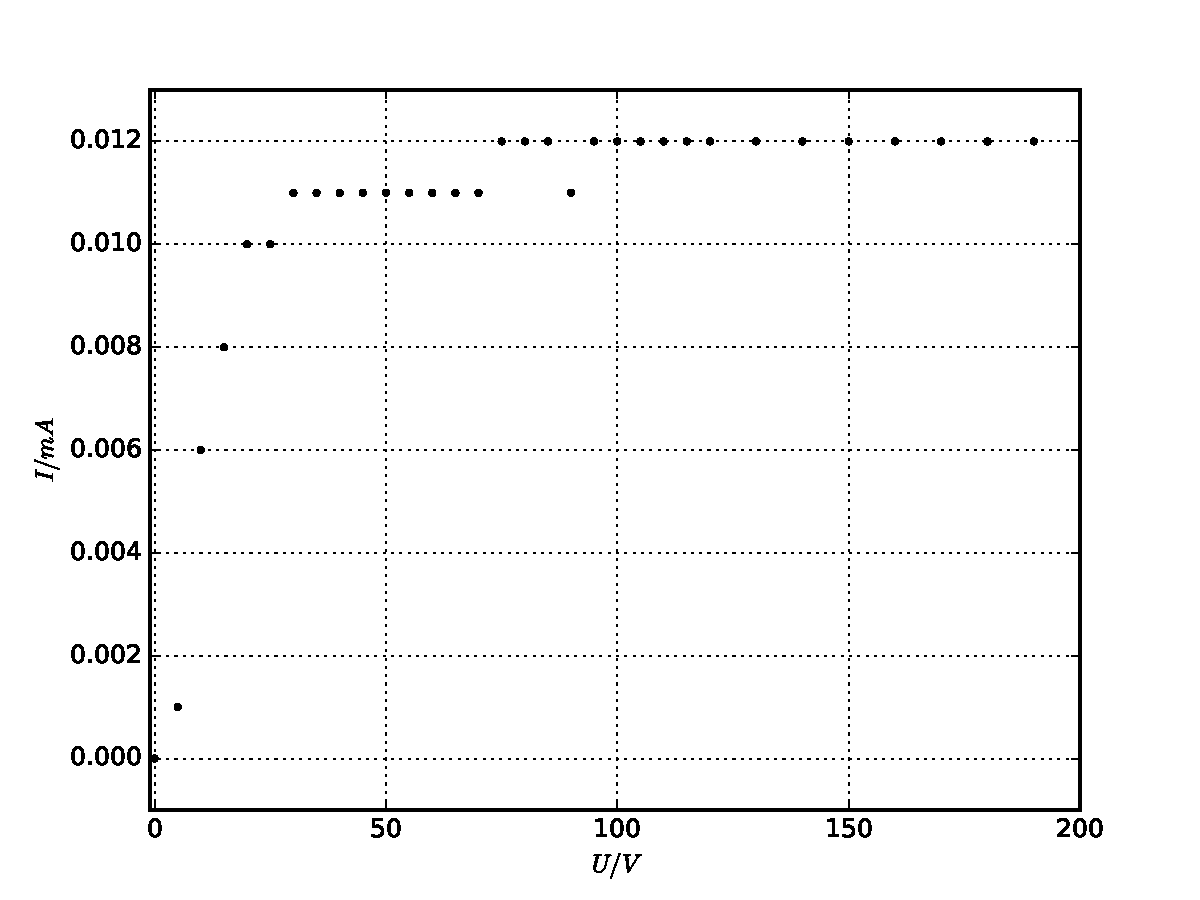
\includegraphics[height=7cm]{./plots/Plot1.pdf}
  \caption{Kennlinie der Diode, aufgenommen bei $U_h = \SI{3.5}{\volt}$, $I_h = \SI{1.8}{\ampere}$}
  \label{fig:Plot1}
\end{figure}

\begin{figure}
  \centering
  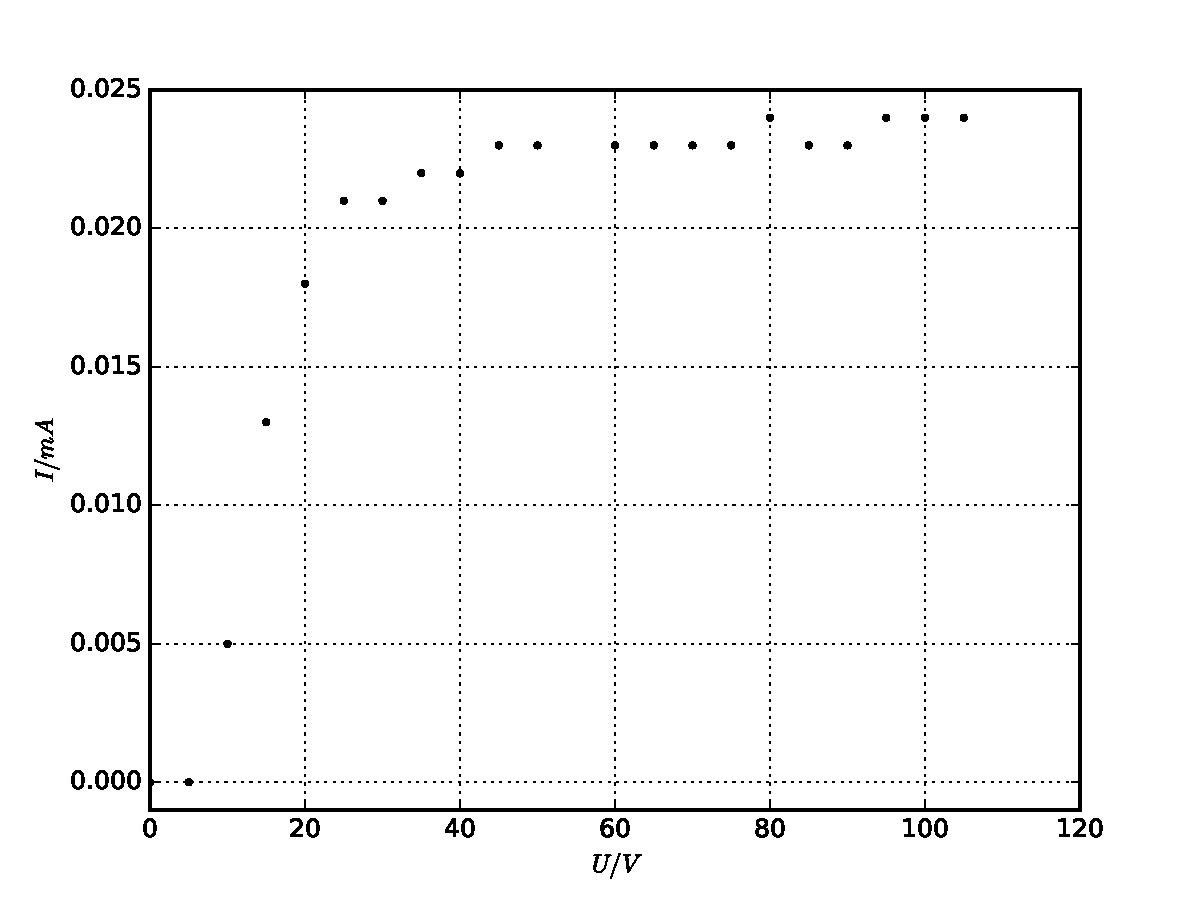
\includegraphics[height=7cm]{./plots/Plot2.pdf}
  \caption{Kennlinie der Diode, aufgenommen bei $U_h = \SI{4}{\volt}$, $I_h = \SI{1.9}{\ampere}$}
  \label{fig:Plot2}
\end{figure}

\begin{figure}
  \centering
  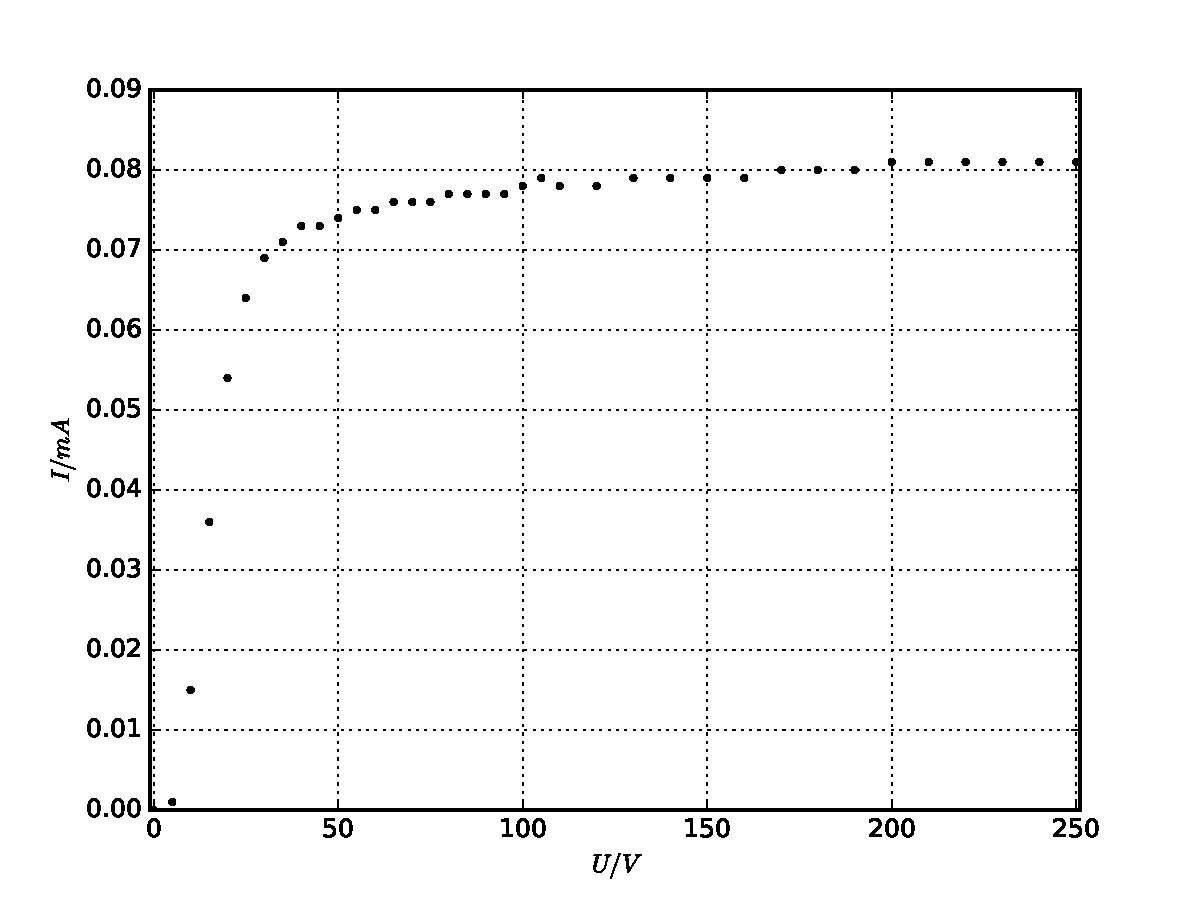
\includegraphics[height=7cm]{./plots/Plot3.pdf}
  \caption{Kennlinie der Diode, aufgenommen bei $U_h = \SI{4.5}{\volt}$, $I_h = \SI{2}{\ampere}$}
  \label{fig:Plot3}
\end{figure}

\begin{figure}
  \centering
  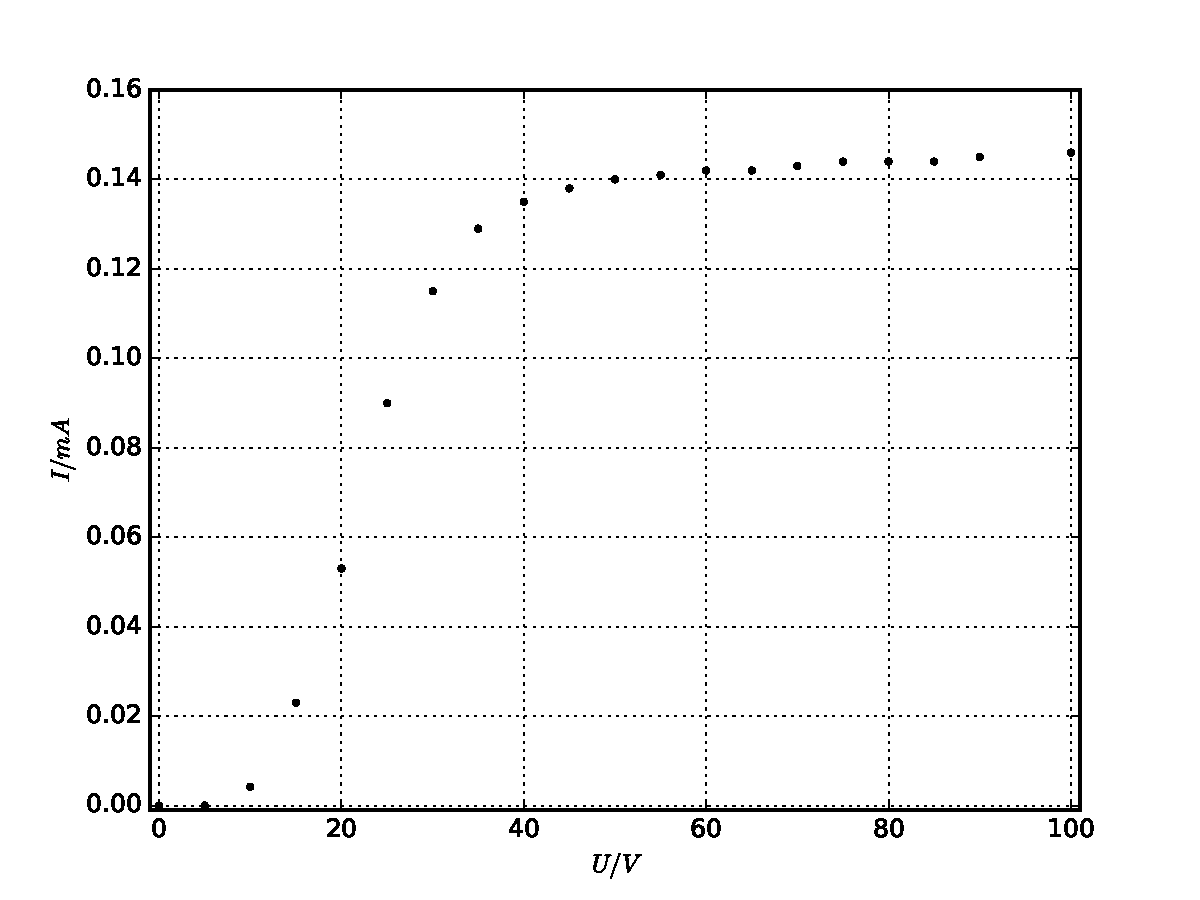
\includegraphics[height=7cm]{./plots/Plot4.pdf}
  \caption{Kennlinie der Diode, aufgenommen bei $U_h = \SI{4.5}{\volt}$, $I_h = \SI{2.1}{\ampere}$}
  \label{fig:Plot4}
\end{figure}

\begin{figure}
  \centering
  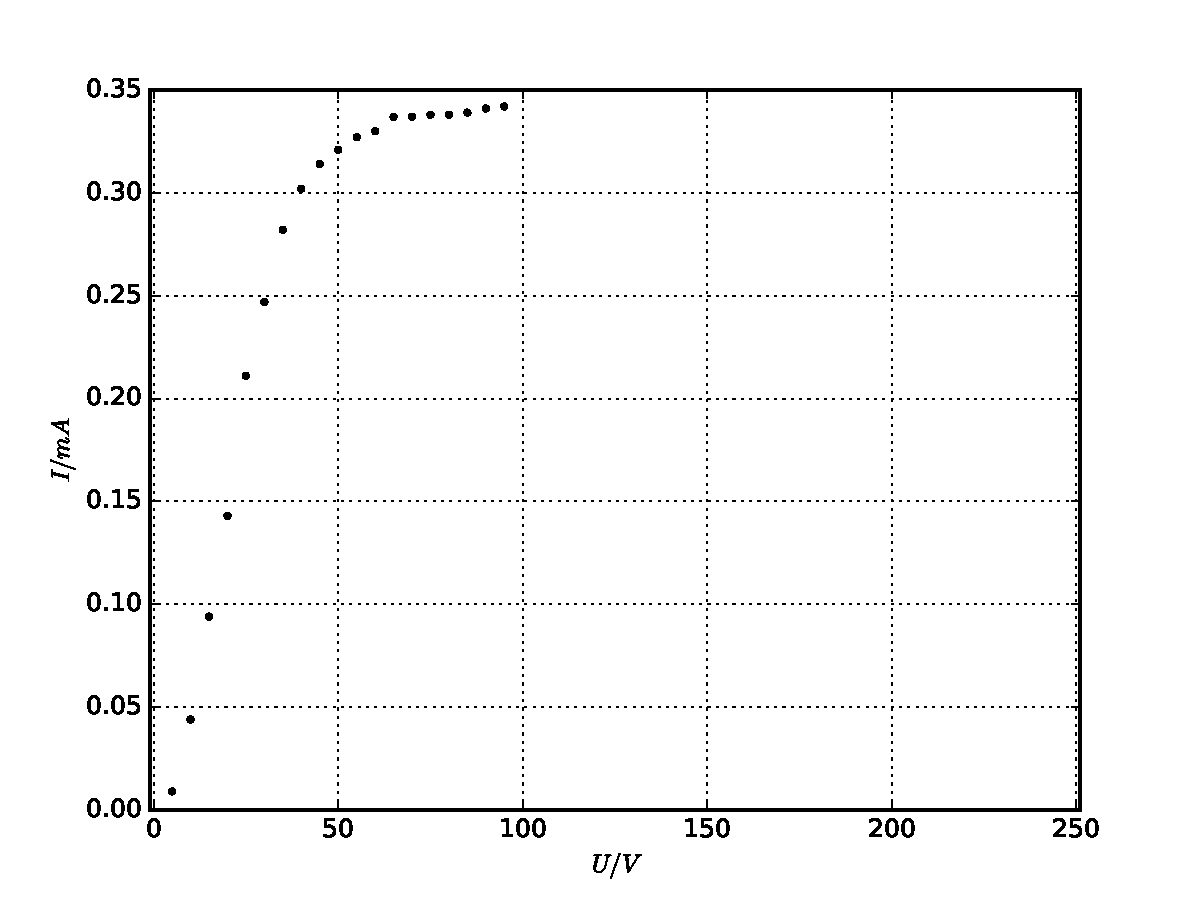
\includegraphics[height=7cm]{./plots/Plot5.pdf}
  \caption{Kennlinie der Diode, aufgenommen bei $U_h = \SI{5}{\volt}$, $I_h = \SI{2.2}{\ampere}$}
  \label{fig:Plot5}
\end{figure}

\begin{table}
  \centering
  \sisetup{round-mode = places, round-precision = 0, scientific-notation = fixed, fixed-exponent = 0}
  \caption{Messwerte der ersten Messreihe}
  \label{tab:Reihe1}
  \begin{tabular}{|S[round-precision = 0]|S[round-precision = 3]|}
    \toprule
    $U/\si{\volt}$ & $I/\si{\milli \ampere}$ \\
    \midrule
    0.000000000000000000e+00 & 0.000000000000000000e+00\\
    5.000000000000000000e+00 & 1.000000000000000021e-0\\
    10.00000000000000000e+0 & 6.000000000000000125e-0\\
    15.00000000000000000e+0 & 8.000000000000000167e-0\\
    20.00000000000000000e+0 & 10.00000000000000021e-0\\
    25.00000000000000000e+0 & 10.00000000000000021e-0\\
    30.00000000000000000e+0 & 10.99999999999999936e-0\\
    35.00000000000000000e+0 & 10.99999999999999936e-0\\
    40.00000000000000000e+0 & 10.99999999999999936e-0\\
    45.00000000000000000e+0 & 10.99999999999999936e-0\\
    50.00000000000000000e+0 & 10.99999999999999936e-0\\
    55.00000000000000000e+0 & 10.99999999999999936e-0\\
    60.00000000000000000e+0 & 10.99999999999999936e-0\\
    65.00000000000000000e+0 & 10.99999999999999936e-0\\
    70.00000000000000000e+0 & 10.99999999999999936e-0\\
    75.00000000000000000e+0 & 12.00000000000000025e-0\\
    80.00000000000000000e+0 & 12.00000000000000025e-0\\
    85.00000000000000000e+0 & 12.00000000000000025e-0\\
    90.00000000000000000e+0 & 10.99999999999999936e-0\\
    95.00000000000000000e+0 & 12.00000000000000025e-0\\
    100.0000000000000000e+0 & 12.00000000000000025e-0\\
    105.0000000000000000e+0 & 12.00000000000000025e-0\\
    110.0000000000000000e+0 & 12.00000000000000025e-0\\
    115.0000000000000000e+0 & 12.00000000000000025e-0\\
    120.0000000000000000e+0 & 12.00000000000000025e-0\\
    130.0000000000000000e+0 & 12.00000000000000025e-0\\
    140.0000000000000000e+0 & 12.00000000000000025e-0\\
    150.0000000000000000e+0 & 12.00000000000000025e-0\\
    160.0000000000000000e+0 & 12.00000000000000025e-0\\
    170.0000000000000000e+0 & 12.00000000000000025e-0\\
    180.0000000000000000e+0 & 12.00000000000000025e-0\\
    190.0000000000000000e+0 & 12.00000000000000025e-0\\
    \bottomrule
  \end{tabular}
\end{table}

\begin{table}
  \centering
  \sisetup{round-mode = places , scientific-notation = fixed, round-precision = 3, fixed-exponent = 0}
  \caption{Messwerte der zweiten Messreihe}
  \label{tab:Reihe2}
  \begin{tabular}{|S|S|}
    \toprule
    $U/\si{\volt}$ & $I/\si{\ampere}$ \\
    \midrule
    0.000000000000000000e+00 & 0.000000000000000000e+00\\
    5.000000000000000000e+00 & 0.000000000000000000e+00\\
    1.000000000000000000e+01 & 5.000000000000000104e-03\\
    1.500000000000000000e+01 & 1.299999999999999940e-02\\
    2.000000000000000000e+01 & 1.799999999999999864e-02\\
    2.500000000000000000e+01 & 2.100000000000000130e-02\\
    3.000000000000000000e+01 & 2.100000000000000130e-02\\
    3.500000000000000000e+01 & 2.199999999999999872e-02\\
    4.000000000000000000e+01 & 2.199999999999999872e-02\\
    4.500000000000000000e+01 & 2.299999999999999961e-02\\
    5.000000000000000000e+01 & 2.299999999999999961e-02\\
    6.000000000000000000e+01 & 2.299999999999999961e-02\\
    6.500000000000000000e+01 & 2.299999999999999961e-02\\
    7.000000000000000000e+01 & 2.299999999999999961e-02\\
    7.500000000000000000e+01 & 2.299999999999999961e-02\\
    8.000000000000000000e+01 & 2.400000000000000050e-02\\
    8.500000000000000000e+01 & 2.299999999999999961e-02\\
    9.000000000000000000e+01 & 2.299999999999999961e-02\\
    9.500000000000000000e+01 & 2.400000000000000050e-02\\
    1.000000000000000000e+02 & 2.400000000000000050e-02\\
    1.050000000000000000e+02 & 2.400000000000000050e-02\\
    \bottomrule
  \end{tabular}
\end{table}

\begin{table}
  \centering
  \sisetup{round-mode = places , scientific-notation = fixed, round-precision = 3, fixed-exponent = 0}
  \caption{Messwerte der dritten Messreihe}
  \label{tab:Reihe3}
  \begin{tabular}{|S|S|}
    \toprule
    $U/\si{\volt}$ & $I/\si{\ampere}$ \\
    \midrule
    0.000000000000000000e+00 & 0.000000000000000000e+00\\
    5.000000000000000000e+00 & 1.000000000000000021e-03\\
    1.000000000000000000e+01 & 1.499999999999999944e-02\\
    1.500000000000000000e+01 & 3.599999999999999728e-02\\
    2.000000000000000000e+01 & 5.399999999999999939e-02\\
    2.500000000000000000e+01 & 6.400000000000000133e-02\\
    3.000000000000000000e+01 & 6.900000000000000577e-02\\
    3.500000000000000000e+01 & 7.099999999999999367e-02\\
    4.000000000000000000e+01 & 7.299999999999999545e-02\\
    4.500000000000000000e+01 & 7.299999999999999545e-02\\
    5.000000000000000000e+01 & 7.399999999999999634e-02\\
    5.500000000000000000e+01 & 7.499999999999999722e-02\\
    6.000000000000000000e+01 & 7.499999999999999722e-02\\
    6.500000000000000000e+01 & 7.599999999999999811e-02\\
    7.000000000000000000e+01 & 7.599999999999999811e-02\\
    7.500000000000000000e+01 & 7.599999999999999811e-02\\
    8.000000000000000000e+01 & 7.699999999999999900e-02\\
    8.500000000000000000e+01 & 7.699999999999999900e-02\\
    9.000000000000000000e+01 & 7.699999999999999900e-02\\
    9.500000000000000000e+01 & 7.699999999999999900e-02\\
    1.000000000000000000e+02 & 7.799999999999999989e-02\\
    1.050000000000000000e+02 & 7.900000000000000078e-02\\
    1.100000000000000000e+02 & 7.799999999999999989e-02\\
    1.200000000000000000e+02 & 7.799999999999999989e-02\\
    1.300000000000000000e+02 & 7.900000000000000078e-02\\
    1.400000000000000000e+02 & 7.900000000000000078e-02\\
    1.500000000000000000e+02 & 7.900000000000000078e-02\\
    1.600000000000000000e+02 & 7.900000000000000078e-02\\
    1.700000000000000000e+02 & 8.000000000000000167e-02\\
    1.800000000000000000e+02 & 8.000000000000000167e-02\\
    1.900000000000000000e+02 & 8.000000000000000167e-02\\
    2.000000000000000000e+02 & 8.100000000000000255e-02\\
    2.100000000000000000e+02 & 8.100000000000000255e-02\\
    2.200000000000000000e+02 & 8.100000000000000255e-02\\
    2.300000000000000000e+02 & 8.100000000000000255e-02\\
    2.400000000000000000e+02 & 8.100000000000000255e-02\\
    2.500000000000000000e+02 & 8.100000000000000255e-02\\
    \bottomrule
  \end{tabular}
\end{table}

\begin{table}
  \centering
  \sisetup{round-mode = places, scientific-notation = fixed, round-precision = 3, fixed-exponent = 0}
  \caption{Messwerte der vierten Messreihe}
  \label{tab:Reihe4}
  \begin{tabular}{|S|S|}
    \toprule
    $U/\si{\volt}$ & $I/\si{\ampere}$ \\
    \midrule
    0.000000000000000000e+00 & 0.000000000000000000e+00\\
    5.000000000000000000e+00 & 0.000000000000000000e+00\\
    1.000000000000000000e+01 & 4.199999999999999740e-03\\
    1.500000000000000000e+01 & 2.299999999999999961e-02\\
    2.000000000000000000e+01 & 5.299999999999999850e-02\\
    2.500000000000000000e+01 & 8.999999999999999667e-02\\
    3.000000000000000000e+01 & 1.150000000000000050e-01\\
    3.500000000000000000e+01 & 1.290000000000000036e-01\\
    4.000000000000000000e+01 & 1.350000000000000089e-01\\
    4.500000000000000000e+01 & 1.380000000000000115e-01\\
    5.000000000000000000e+01 & 1.400000000000000133e-01\\
    5.500000000000000000e+01 & 1.409999999999999865e-01\\
    6.000000000000000000e+01 & 1.419999999999999873e-01\\
    6.500000000000000000e+01 & 1.419999999999999873e-01\\
    7.000000000000000000e+01 & 1.429999999999999882e-01\\
    7.500000000000000000e+01 & 1.439999999999999891e-01\\
    8.000000000000000000e+01 & 1.439999999999999891e-01\\
    8.500000000000000000e+01 & 1.439999999999999891e-01\\
    9.000000000000000000e+01 & 1.449999999999999900e-01\\
    1.000000000000000000e+02 & 1.459999999999999909e-01\\
    \bottomrule
  \end{tabular}
\end{table}

\begin{table}
  \centering
  \sisetup{round-mode = places , scientific-notation = fixed, round-precision = 3, fixed-exponent = 0}
  \caption{Messwerte der fünften Messreihe}
  \label{tab:Reihe5}
  \begin{tabular}{|S|S|}
    \toprule
    $U/\si{\volt}$ & $I/\si{\ampere}$ \\
    \midrule
    5.000000000000000000e+00 & 8.999999999999999320e-03\\
    1.000000000000000000e+01 & 4.399999999999999745e-02\\
    1.500000000000000000e+01 & 9.400000000000000022e-02\\
    2.000000000000000000e+01 & 1.429999999999999882e-01\\
    2.500000000000000000e+01 & 2.109999999999999931e-01\\
    3.000000000000000000e+01 & 2.469999999999999973e-01\\
    3.500000000000000000e+01 & 2.819999999999999729e-01\\
    4.000000000000000000e+01 & 3.019999999999999907e-01\\
    4.500000000000000000e+01 & 3.140000000000000013e-01\\
    5.000000000000000000e+01 & 3.210000000000000075e-01\\
    5.500000000000000000e+01 & 3.270000000000000129e-01\\
    6.000000000000000000e+01 & 3.300000000000000155e-01\\
    6.500000000000000000e+01 & 3.370000000000000218e-01\\
    7.000000000000000000e+01 & 3.370000000000000218e-01\\
    7.500000000000000000e+01 & 3.380000000000000226e-01\\
    8.000000000000000000e+01 & 3.380000000000000226e-01\\
    8.500000000000000000e+01 & 3.390000000000000235e-01\\
    9.000000000000000000e+01 & 3.410000000000000253e-01\\
    9.500000000000000000e+01 & 3.420000000000000262e-01\\
    -1.000000000000000021e-02 & 3.000000000000000000e+00\\
    -1.000000000000000056e-01 & 3.100000000000000089e+00\\
    -2.000000000000000111e-01 & 2.399999999999999911e+00\\
    -2.999999999999999889e-01 & 1.600000000000000089e+00\\
    -4.000000000000000222e-01 & 1.399999999999999911e+00\\
    -5.000000000000000000e-01 & 1.250000000000000000e+00\\
    -5.999999999999999778e-01 & 8.100000000000000533e-01\\
    -6.999999999999999556e-01 & 5.699999999999999512e-01\\
    -8.000000000000000444e-01 & 2.999999999999999889e-01\\
    -9.000000000000000222e-01 & 1.600000000000000033e-02\\
    -1.000000000000000000e+00 & 8.099999999999999561e-03\\
    \bottomrule
  \end{tabular}
\end{table}
\FloatBarrier

\subsection{Langmuir-Schottkysches Gesetz}

\begin{figure}
  \centering
  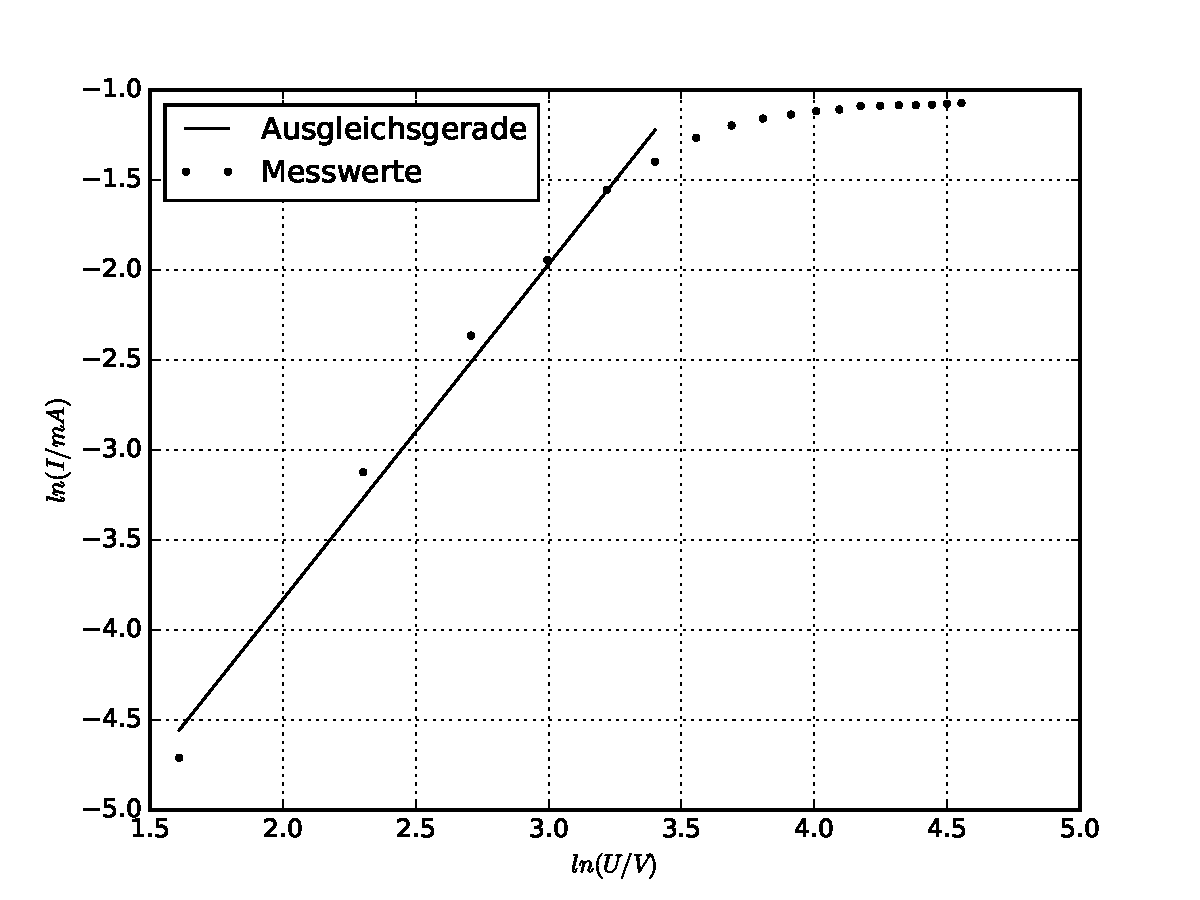
\includegraphics[height=7cm]{./plots/langmuir.pdf}
  \caption{Doppellogaritmische Darstellung der $U_h = \SI{5}{\volt}$, $I_h = \SI{2.2}{\ampere}$-Kennlinie, mit linearem Ausgleich}
  \label{fig:langmuir}
\end{figure}

Die Grenze des Raumladungsgebietes wurde auf $\SI{25}{\volt}$ geschätzt, da in Abb. \ref{fig:langmuir} erkennbar ist, dass dies den Berreich darstellt, in dem der Strom in doppelt logarithmischer Darstellung linear verläuft. Über diese doppelt logarithmierten Werte wird eine lineare Ausgleichsrechnung gemäß
\begin{align*}
  a &= 1.9 \pm  0.1 \\
  b &= -7.6 \pm 0.3
\end{align*}
mit $a$ als Steigung und $b$  als y-Achsenabschnitt durchgeführt.

\subsection{Anlaufstrom und Kathodentemperatur}
 \begin{figure}
   \centering
   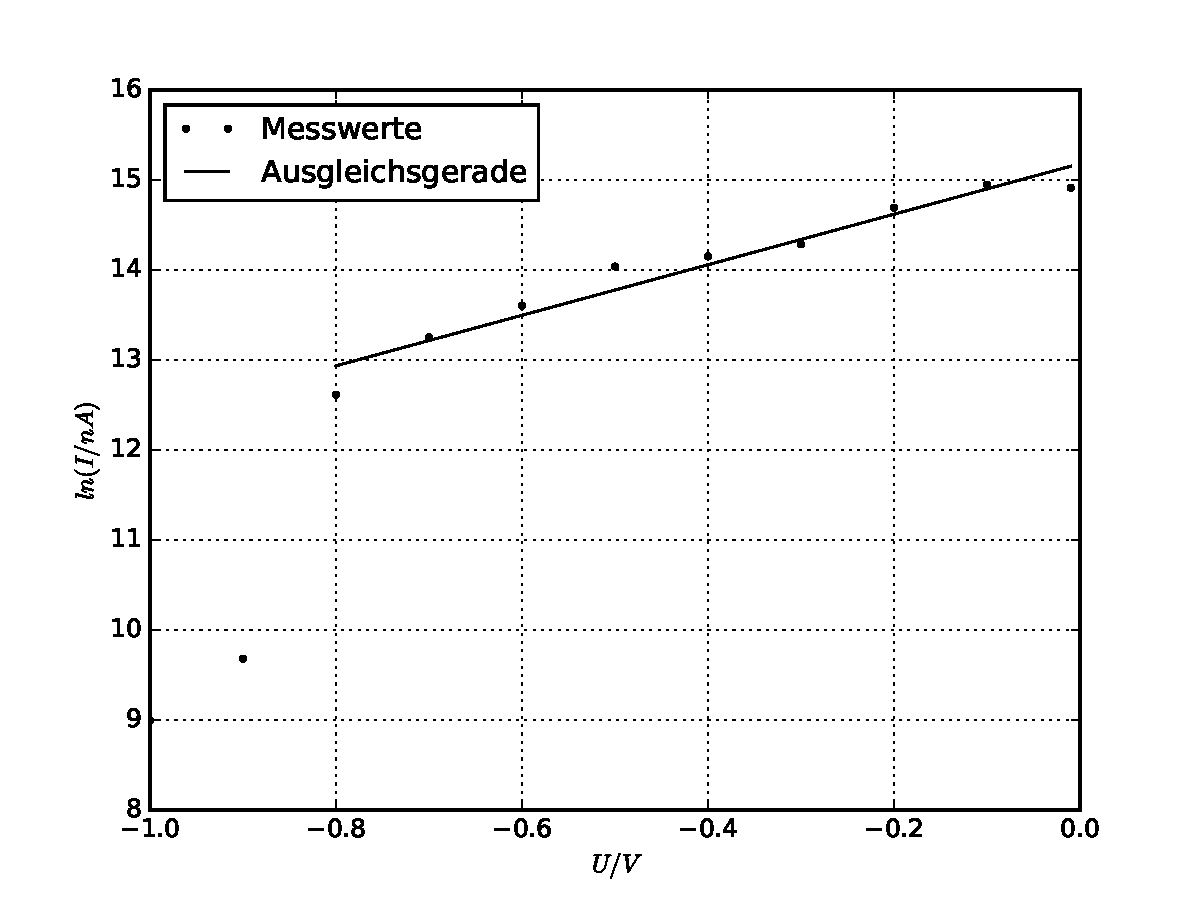
\includegraphics[height = 7cm]{./plots/Plot6.pdf}
   \caption{Logarithmische Darstellung des Anlaufstromes, mit linearem Ausgleich}
   \label{fig:Plot6}
 \end{figure}

Linearer Ausgleich des Anlaufstromes (Abb. \ref{fig:Plot6}) liefert die Werte
\begin{align*}
  a &= 2.8 \pm 0.3 \\
  b &= 15.2 \pm 0.1 \;.
\end{align*}
Aus $a = \frac{e_0}{kT}$ folgt mit $k = \SI{8.7e-5}{\electronvolt \kelvin}$:
\begin{equation*}
  T = \frac{e_0}{k \; a} = \SI{2050 \pm 200}{\kelvin}.
\end{equation*}
Die verwendete Heizleistung beträgt $p = U I = \SI{24.2}{\watt}$.
Die Leistungsbilanz der Apparatur lautet
\begin{equation*}
  I_\text{f} U_\text{f} = f \eta \sigma T^4 + N_\text{WL}
\end{equation*}
mit $N_\text{WL} \approx 1$ als Wärmeableitung der Apparatur, $f = \SI{0.35}{\centi \meter \squared}$ als Kathodenfläche der verwendeten Diode (Diode 2) und $\eta = 0.28$ als Wärmeemissionsgrad der Fläche. Diese Bilanz liefert
\begin{align*}
  T_1 &= \SI{1755}{\kelvin} \\
  T_2 &= \SI{1854}{\kelvin} \\
  T_3 &= \SI{1945}{\kelvin} \\
  T_4 &= \SI{1972}{\kelvin} \\
  T_5 &= \SI{2057}{\kelvin}.
\end{align*}
Die Standardabweichungen sind hierbei vernachlässigbar klein.

\subsection{Austrittsarbeit der Kathode}

 Über die Richardson Gleichung ergeben sich mit den Temperaturen der Kathode die äußeren Potentiale
 \begin{align*}
   \phi_1 &= \SI{4.28}{\electronvolt} \\
   \phi_2 &= \SI{4.53}{\electronvolt} \\
   \phi_3 &= \SI{4.76}{\electronvolt} \\
   \phi_4 &= \SI{4.82}{\electronvolt} \\
   \phi_5 &= \SI{5.03}{\electronvolt}.
 \end{align*}
Mittelung ergibt $\phi =  \SI{4.68 \pm 0.13}{\electronvolt}$.
